\chapter{Grenze}

\section{Das Ganze und die Grenze}

Brentano unterscheidet zwei Arten des Kontinuierlichen nach der Weise, wie sie bestehen. Das topisch Kontinuierliche, der Körper, besteht dem Ganzen nach: Alle seine Teile sind zugleich da. Das chronisch Kontinuierliche, das Verlaufende, besteht nur einer Grenze nach. Von einer Melodie ist immer nur ein Ton wirklich, von einer Bewegung nur eine Lage. Was vorher war, ist nicht mehr, was nachher kommt, ist noch nicht. Das Jetzt ist also Grenze eines Kontinuums, das im Übrigen nicht besteht.\footnote{Brentano, Philosophische Untersuchungen zu Raum, Zeit und Kontinuum, Erster Teil, Kapitel zum Kontinuierlichen.}

Man könnte einwenden, eine Grenze ohne das Begrenzte sei nichts, und das Jetzt sei deshalb ebenso nichts wie ein Punkt ohne Linie. Brentano nimmt den Einwand auf und wendet ihn. Die innere Wahrnehmung zeigt in recto die Grenze und in obliquo die Strecke, für die der Punkt eine Grenze ist. \zitat{Fragt man, in welcher Länge die Strecke in obliquo vorgestellt und anerkannt werde, so ist zu antworten: in gar keiner bestimmten Länge.}\footnote{Brentano, Untersuchungen, S.\,131.} Das Jetzt ist also nicht die Grenze einer Strecke, die daneben vorhanden wäre, sondern die Grenze einer Strecke, die nur in der Grenze mitgemeint ist, und zwar ohne Maß. Der Raum verhält sich gerade umgekehrt. Er wird als Ganzes vorgestellt, und seine Grenzen, Flächen, Linien, Punkte, werden an ihm gesetzt. Hegel sagt es in der Nachschrift kurz: \zitat{Man kann einem Raume überall Grenzen setzen, den Raum aber nicht unterbrechen.}\footnote{Hegel, Naturphilosophie, Nachschrift, nach Bonsiepen.} Überall, das heißt: an beliebiger Stelle; nicht unterbrechen, das heißt: keine der gesetzten Grenzen ist eine Grenze des Raumes selbst.

Daraus folgt eine Bestimmung des Körpers, die Brentano ausdrücklich zieht: Ein Körper, der in der Zeit besteht, ist die dreidimensionale Grenze eines Kontinuums, das eine Dimension mehr hat, der Zeit. Er besteht nur als diese Grenze. \zitat{Wenn ein Ding, das besteht, beharrt, so geschieht dies durch ein kontinuierlich sich wiederholendes Sich-Erneuern.}\footnote{Brentano, Untersuchungen, Kapitel zum Beharren.} Das Beharren ist also keine Ruhe, sondern eine Tätigkeit ohne Unterschied. Was räumlich als ruhende Substanz erscheint, ist zeitlich ein Erneuern, das sich von Grenze zu Grenze fortsetzt. Hier zeigt sich zum ersten Mal, dass das, was am Raum am festesten scheint, das Beharrliche, seine Weise zu sein von der Zeit hat.

\section{Der wahrhafte Punkt}

Hegel gelangt von der anderen Seite zum selben Ergebnis. Der Punkt soll im Raum die Negation des Raumes sein, das Fürsichsein, der im Raum seiende Gedanke, wie Bonsiepen paraphrasiert. Aber im Raum hat der Punkt keine Wirklichkeit. Sobald er gesetzt ist, ist er Linie, die Linie ist Fläche, die Fläche ist Raum. Die Negation, die der Punkt sein sollte, wird sogleich wieder ausgebreitet. Deshalb heißt es in der Nachschrift: \zitat{Die Zeit ist also erst der wahrhafte Punkt.} In der Zeit hat die Negativität Wirklichkeit: Das Jetzt ist, indem es nicht ist, und darin ist es, was der Punkt im Raum nur sein soll. Was der Punkt im Raum nicht sein kann, ist er als Jetzt; und ein Ort, so lässt sich der Übergang lesen, ist nicht ein Raumteil, sondern ein Punkt, der als Jetzt gesetzt ist, also die Zeit im Raum.\footnote{Koch, Hegelsche Subjekte in Raum und Zeit, zum Übergang des Raumes in die Zeit; Bonsiepen, Hegels Raum-Zeit-Lehre, zu den Nachschriften. Die Bestimmung des Ortes als gesetztes Jetzt ist eigene Lesart des Übergangs, kein Wortlaut Hegels.}

Fink sagt es ohne die Dialektik: Der Raum ist primär Kontinuum, die Zeit ist als Jetzt primär diskret, \zitat{das Diskrete schlechthin}.\footnote{Fink, Frühgeschichte, Kapitel zur aristotelischen Zeit-Analytik.} Man kann die Ausdehnung des Raumes teilen, aber die Teilung kommt zum Raum hinzu; das Jetzt kommt zur Zeit nicht hinzu, es ist die Weise, wie sie ist.

\section{Ein Widerspruch, der keiner ist}

Nun sagt Baumann das Gegenteil. Für ihn ist gerade das Diskrete, das Abgesetzte in der Zeit \emph{nicht}; die Zeit ist \zitat{nicht aus Momenten als aus Theilen zusammengesetzt}, und die Zahl gehört mehr dem Raum als der Zeit.\footnote{Baumann, Lehren, Bd.\,2, S.\,658--668.} Guzzoni bestätigt ihn von einer ganz anderen Seite: Es gibt keine halbe und keine doppelte Weile. Eine Weile ist eine Phase der Zeit, die nicht als Abfolge von Jetztpunkten erfahren wird, und ihre Dauer ist nur qualitativ bestimmt.\footnote{Guzzoni, Weile und Weite, Kapitel zur Weile.} Wer die Zeit teilt, wie man den Raum teilt, in Abschnitte gleicher Länge, hat sie schon nach dem Raum behandelt.

Fink und Baumann widersprechen einander nur, wenn man \zitat{diskret} in beiden Sätzen gleich versteht. Sie meinen aber zwei Dinge. Fink meint den einen Schnitt, der die Zeit ist: das Jetzt, vor dem alles vergangen und nach dem alles künftig ist. Baumann meint die vielen Schnitte, die man an einer Linie anbringen kann, um sie in Teile zu zerlegen. Die Zeit hat den einen und nicht die vielen. Der Raum hat die vielen und nicht den einen. Brentano hat diese Kreuzung ausgesprochen, ohne sie als solche zu benennen: \zitat{Bei der Zeit [\ldots] ist dieser Punkt der Sache nach ein ausgezeichneter. Beim Raum gibt es keinen Punkt, der in ähnlicher Weise sich der Sache nach unterschiede.}\footnote{Brentano, Untersuchungen, S.\,117.}

\begin{figure}[htbp]
\centering
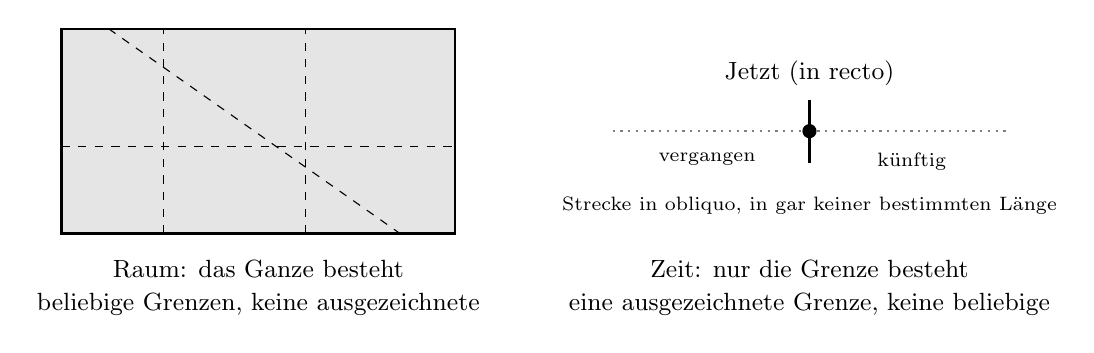
\begin{tikzpicture}[scale=1]
% --- Raum: das Ganze besteht, beliebige Grenzen ---
\begin{scope}
\fill[gray!20] (0,0) rectangle (5,2.6);
\draw[thick] (0,0) rectangle (5,2.6);
\draw[dashed] (1.3,0) -- (1.3,2.6);
\draw[dashed] (3.1,0) -- (3.1,2.6);
\draw[dashed] (0,1.1) -- (5,1.1);
\draw[dashed] (0.6,2.6) -- (4.3,0);
\node at (2.5,-0.45) {\small Raum: das Ganze besteht};
\node at (2.5,-0.9) {\small beliebige Grenzen, keine ausgezeichnete};
\end{scope}
% --- Zeit: nur die Grenze besteht ---
\begin{scope}[xshift=7cm]
\draw[dotted,thick,gray] (0,1.3) -- (2.4,1.3);
\draw[dotted,thick,gray] (2.6,1.3) -- (5,1.3);
\fill (2.5,1.3) circle (0.09);
\draw[thick] (2.5,0.9) -- (2.5,1.7);
\node[above] at (2.5,1.75) {\small Jetzt (in recto)};
\node[below] at (1.2,1.15) {\scriptsize vergangen};
\node[below] at (3.8,1.15) {\scriptsize künftig};
\node at (2.5,0.35) {\scriptsize Strecke in obliquo, \zitat{in gar keiner bestimmten Länge}};
\node at (2.5,-0.45) {\small Zeit: nur die Grenze besteht};
\node at (2.5,-0.9) {\small eine ausgezeichnete Grenze, keine beliebige};
\end{scope}
\end{tikzpicture}
\caption{Ganzes und Grenze. Links das topisch Kontinuierliche, das dem Ganzen nach besteht und überall Grenzen zulässt; rechts das chronisch Kontinuierliche, das nur als eine Grenze besteht, deren Strecke ohne Maß mitgemeint ist (nach Brentano). Die beiden Weisen, diskret zu sein, kreuzen sich: ein ausgezeichneter Schnitt ohne beliebige, beliebige Schnitte ohne ausgezeichneten.}
\label{abb:grenze}
\end{figure}

Damit ist die erste Asymmetrie bestimmt. Sie liegt nicht darin, dass die Zeit \zitat{diskret} und der Raum \zitat{kontinuierlich} wäre oder umgekehrt. Beide sind kontinuierlich, und beide lassen sich unterbrechen, aber auf zwei einander ausschließende Weisen. Die Zeit hat ihre Grenze an sich selbst, an genau einer Stelle, und diese Stelle wandert nicht, sondern ist immer dieselbe, das Jetzt, das sich erneuert. Der Raum hat keine Grenze an sich selbst; sie wird ihm gesetzt, an beliebiger Stelle, und keine der Stellen ist vor der anderen ausgezeichnet.

\section{Wo der Raum seine Grenze herhat}

Wenn der Raum von sich aus keine ausgezeichnete Grenze hat, woher hat er dann die, die er offenbar hat? Denn es gibt Orte, und ein Ort ist etwas anderes als eine beliebige Stelle. Die Antwort, die sich aus Hegels Übergang ergibt: Der Ort ist ein als Jetzt gesetzter Punkt. Das ausgezeichnete Hier ist die Zeit, die sich an einer Stelle des Raumes niedergelassen hat. Kochs Antwort ergänzt sie: Das ausgezeichnete Hier ist der Ort des Leibes. Beide Antworten sagen dasselbe, wenn man bedenkt, dass der Leib das Zeitliche ist, das im Raum ist. Er ist nach Brentano die dreidimensionale Grenze eines zeitlichen Kontinuums, das sich in ihm erneuert; er ist nach Koch das Partikulare, das sich a priori selbst individuiert und lokalisiert.

Was also im Raum Grenze ist, im ausgezeichneten Sinn, ist geliehene Zeit. Die Geometrie kennt diese Grenze nicht, und sie braucht sie nicht, denn sie setzt ihre Grenzen überall. Dass es im Raum ein Hier gibt, das kein Dort ist, verdankt sich nicht dem Raum. Das ist das erste Ergebnis, und ihm ist nun in seine beiden Richtungen nachzugehen: zum Hier, das der Leib besetzt, und zum Jetzt, das nach Fink \zitat{weltweit} sein soll.
